\documentclass[11pt]{article}

\usepackage[T1]{fontenc}
\usepackage{lmodern}
\usepackage[margin=1in]{geometry}
\usepackage{microtype}
\usepackage{amsmath}
\usepackage{booktabs}
\usepackage{graphicx}
\usepackage{caption}
\usepackage{float}
\usepackage{enumitem}
\usepackage{xcolor}
\usepackage{tikz}
\usepackage[round,authoryear]{natbib}
\usepackage[hidelinks]{hyperref}

\definecolor{accent}{HTML}{1F44D6}
\captionsetup{font=small,labelfont=bf}
\setlist{itemsep=2pt,topsep=4pt}
\newcommand{\m}{\ensuremath{-}}

\title{Copying Congress After Disclosure:\\A Pre-Specified Event Study of Congressional Purchases, 2020--2025}
\author{Yinka Vaughan\\
\small Wesleyan University\\
\small ORCID \href{https://orcid.org/0009-0005-8933-5396}{0009-0005-8933-5396}}
\date{November 2026\\[2pt]\small Working paper}

\begin{document}
\maketitle

\begin{abstract}
\noindent Members of the US Congress must disclose their stock trades within 45 days. I ask whether an outside investor who buys what members bought, once the purchase is disclosed, earns an abnormal return. Using 3,942 purchases of US common stock by 124 House members from 2020 to 2025, I form a portfolio that buys each stock on the first trading day after its purchase is disclosed and holds it for 62 trading days. This test, specified before any return was estimated for this study, gives a Carhart four-factor alpha of \m1.63\% a year ($t = \m0.66$, $p = 0.51$), with a 95\% confidence interval from \m6.5\% to +3.2\% a year. The result holds across alternative holding periods, factor models and samples, and none of the planned event-level tests yields a statistically significant abnormal return after correction for multiple testing. Across all House trades in the sample, the median trade was disclosed 13 days after it was made, and 6.6\% were disclosed more than 45 days after the trade.

\medskip
\noindent\textbf{Keywords:} congressional trading, STOCK Act, event study, calendar-time portfolio, abnormal returns, disclosure\\
\textbf{JEL:} G11, G14, G18
\end{abstract}

\section{Introduction}

Since the STOCK Act of 2012, members of Congress have had to report covered securities transactions over \$1,000 by themselves, their spouses and their dependent children within 30 days of learning of the transaction and no later than 45 days after it \citep{stockact2012,houseethics2026}. The reports are public. Anyone who believes that members trade on information the market does not have can wait for a report and buy what the member bought.

Whether that strategy works depends on returns after the report, not after the trade. A member who knows something on the trade date may profit, but an outside investor sees the trade only when it is disclosed, by which time part or all of any information may already be in the price. Most studies of congressional trading measure returns from the trade date, which describes performance from the member's own entry point. This paper measures them from the disclosure date, the first day an outside investor could act.

I study 3,942 House purchases of US common stock made from January 2020 to December 2025 and disclosed within a year. Returns come from CRSP and risk adjustment from the Fama--French three factors plus momentum. The primary test is a calendar-time portfolio: each day it holds every stock bought by a member and disclosed in the previous 62 trading days, and its four-factor intercept is the copy strategy's alpha. I also estimate event-level cumulative abnormal returns (CARs) from the trade date and from the disclosure date at three horizons, with standard errors clustered by member and by month and a Holm correction across the six tests.

The sample rules, the price source, the factor model, the primary test and the multiple-testing correction were written into a plan and committed to the project's public repository before any return was computed for this analysis. An earlier version of the project had estimated returns with a different method; Appendix~\ref{app:earlier} explains why that estimate is withdrawn. Section~\ref{sec:plan} lists the departures from the plan, including an estimation change made after the first run and an entry-timing correction made after an outside review.

The copy portfolio earns no detectable alpha. At the primary 62-day holding period the annualized four-factor alpha is \m1.63\% ($t = \m0.66$), and the 95\% confidence interval excludes alphas above about 3.2\% a year. None of the six planned CARs differs from zero after the Holm correction, and none of seven robustness checks is significant. The largest positive estimate weights each stock by its disclosed dollar amount (7.19\% a year, $t = 1.45$).

Most studies of congressional trades made since 2012 have found no abnormal returns (Section~\ref{sec:literature}). The closest recent ones measure returns from the trade date, so they leave open whether any return remains after the trades become public. I test that directly, using a calendar-time portfolio formed after disclosure and data through 2025. Because the delay between trade and report is what separates the two questions, I also measure how long House members took to disclose and how often they exceeded the 45-day limit.

\section{Prior evidence}\label{sec:literature}

Studies of the years before the STOCK Act disagree. \citet{ziobrowski2004senate} and \citet{ziobrowski2011house} find that portfolios mimicking senators' and House members' purchases beat the market in samples running from the mid-1980s to 2001. \citet{eggers2013capitol} revisit both studies and analyze 2004 to 2008; they find no information advantage in either period, and the average member would have done better in an index fund. \citet{eggers2014political} find that members' holdings in local firms and in campaign contributors do better than their other holdings. \citet{karadas2019trading} and \citet{huang2016trading} find abnormal returns in the years just before the Act and none after it.

Studies using post-2012 trades generally find no abnormal returns. \citet{belmont2020relief} hand-collect senators' trades from 2012 to March 2020, measure buy-and-hold abnormal returns from the trade date, and find that purchases slightly underperform industry-and-size benchmarks; a calendar-time Carhart regression of a trade-size-weighted portfolio, also built from trade dates, gives an insignificant alpha. A later version was published as \citet{belmont2022senators}. \citet{fischer2025democracy} extend that data set to 2023 with House and Senate trades by 331 members and focus on the 15 most active traders. Measuring buy-and-hold abnormal returns from the purchase date at 20, 60 and 127 days, they find that Congress does not significantly outperform in any period, although mean abnormal returns are somewhat higher from 2020 to 2023. \citet{zhou2026illusion} finds no abnormal returns on trades in firms within the jurisdiction of a member's committees.

The two closest studies both measure returns from the trade date. Mean buy-and-hold abnormal returns over long horizons have skewed distributions and overlapping, cross-correlated windows, and their test statistics can be badly misspecified \citep{lyon1999improved,mitchell2000managerial}. A calendar-time portfolio regression avoids both problems \citep{fama1998market}. I use one, from the disclosure date, as the single confirmatory test.

\section{Data}\label{sec:data}

\subsection{Trades}

Trades come from a snapshot of the House and Senate Stock Watcher data sets, which transcribe the periodic transaction reports that members file with the Clerk of the House and the Secretary of the Senate. The project's pipeline pulled those data sets and scraped the official disclosure sites where a record was missing. The snapshot was committed to the project repository on 6 April 2026 and has 16,202 rows. The upstream data sets are no longer reachable, so the snapshot is the only copy of this extract; it is archived with the code, with a test that fails if its hash changes.

Each row gives the member, the owner (the member, a spouse, a dependent child, or joint), the ticker, the transaction type, the transaction date, the amount as one of the bands the law allows, and, for House rows, the disclosure date. Senate rows in the snapshot carry no disclosure date. Senate purchases therefore enter only the trade-date analyses.

An event is a purchase of a listed common stock by a member, spouse or dependent with a transaction date from 1 January 2020 to 31 December 2025. Rows that repeat the same member, owner, ticker, transaction date and amount band are collapsed into one event. For the disclosure-date analyses, the disclosure must fall on or after the trade and no more than 365 days later; the 12 purchases disclosed before their trade and the 45 disclosed more than a year later are treated as data errors.

\subsection{Prices and factors}

Daily returns come from the CRSP daily stock file in the CIZ format, accessed through Wharton Research Data Services, with data through 31 December 2025 \citep{crsp2026daily}. A ticker is matched to the CRSP security whose name-history record covers the transaction date, since tickers move between firms. The match is restricted to common stock: equity securities of subtype common with ordinary shares. ADRs are excluded because the factors are built from US common stocks. In 14 events two CRSP common-stock records cover the trade date, and the lower permanent identifier is kept. CRSP's CIZ returns include the delisting return, so stocks that delist inside a window keep their final return.

Factors are the daily Fama--French market, size and value factors and the momentum factor, with the one-month Treasury bill rate, from Kenneth French's data library, downloaded on 12 November 2026 \citep{fama1993common,carhart1997persistence,french2026data}. The five-factor robustness check uses the daily \citet{fama2015five} factors from the same library, downloaded the same day.

\subsection{Sample}

Table~\ref{tab:flow} shows how the sample is built. Of the 5,137 purchases that pass the trade rules, 4,456 match a CRSP common stock on the trade date: 3,996 House and 460 Senate purchases by 136 members in 1,011 securities. Most of the 365 purchases with no CRSP record are exchange-traded funds and trusts, over-the-counter foreign shares, and closed-end funds; none of the most frequent ones is a listed US common stock under a wrong ticker. The primary test uses the 3,942 matched House purchases with a valid disclosure date, made by 124 members in 959 stocks. In that sample the median purchase was disclosed 15 days after the trade, the members themselves own 1,861 of the purchases, and the five most active members account for 33.5\%. Because CRSP data end on 31 December 2025, 39 of the 3,942 purchases were disclosed too late to enter the portfolio, and another 237 are held for fewer than 62 trading days.

\begin{table}[t]
\centering
\caption{Sample construction}\label{tab:flow}
\begin{tabular}{lr}
\toprule
Step & Events \\
\midrule
Rows in the trade snapshot & 16,202 \\
Purchases & 7,722 \\
With a valid ticker & 5,652 \\
Stock (no options or other securities) & 5,545 \\
Transaction date 2020-01-01 to 2025-12-31 & 5,162 \\
After removing duplicates & 5,137 \\
\quad No CRSP common stock or ADR record on the trade date & 365 \\
\quad ADRs (excluded) & 191 \\
\quad Other share types (excluded) & 125 \\
Matched to CRSP common stock & 4,456 \\
\quad of which House & 3,996 \\
\quad of which Senate & 460 \\
Matched House purchases disclosed 0 to 365 days after the trade & 3,942 \\
\bottomrule
\end{tabular}

\smallskip
\parbox{0.86\linewidth}{\footnotesize The last row is the sample for the primary test. Before CRSP matching, 4,586 purchases meet the disclosure rule; 494 Senate purchases have no disclosure date, 12 were disclosed before the trade, and 45 more than 365 days after it.}
\end{table}

\section{Method}\label{sec:method}

\subsection{Calendar-time copy portfolio (primary test)}

On each trading day $t$, the copy portfolio holds every stock that a member bought and whose purchase was disclosed within the previous $H$ trading days. A stock enters on the first trading day strictly after the disclosure date, so a purchase disclosed on a Friday, a Saturday or a Sunday enters on Monday, and a filing posted after the close cannot be traded on the same day. It stays for $H$ trading days. Weights are equal by stock, not by purchase: a stock named by several active purchases is held once, with the same weight as every other stock held that day. The portfolio's daily excess return is regressed on the four factors:
\begin{equation}
R_{p,t} - R_{f,t} = \alpha + \beta\,(R_{m,t} - R_{f,t}) + s\,\mathit{SMB}_t + h\,\mathit{HML}_t + m\,\mathit{MOM}_t + \varepsilon_t .
\end{equation}
The intercept $\alpha$ is the daily abnormal return of copying, reported as $252\alpha$. Standard errors are Newey--West with Bartlett weights \citep{newey1987simple} and $\lfloor 4(T/100)^{2/9} \rfloor$ lags \citep{newey1994automatic}, which is 7 lags for the 1,505 days on which the portfolio holds a stock; Table~\ref{tab:extra} repeats the test with 21 and 62 lags. P-values come from the normal distribution. The pre-declared primary test is $H = 62$ trading days, about three calendar months; $H = 20$ and $H = 125$ are secondary.

The calendar-time approach treats the portfolio's daily return as the unit of observation, so overlapping holding periods and purchases that cluster on the same dates do not overstate the evidence \citep{fama1998market,mitchell2000managerial}.

\subsection{Event-level abnormal returns}

For each event $i$ with event date $0$, I estimate the stock's factor loadings by regressing its excess return on the four factors over trading days $-250$ to $-30$, requiring at least 100 returns. Its abnormal return on day $\tau$ removes factor exposure only:
\begin{equation}
AR_{i,\tau} = (R_{i,\tau} - R_{f,\tau}) - \hat\beta_i (R_{m,\tau} - R_{f,\tau}) - \hat s_i\,\mathit{SMB}_\tau - \hat h_i\,\mathit{HML}_\tau - \hat m_i\,\mathit{MOM}_\tau ,
\end{equation}
and $\mathit{CAR}_i(h) = \sum_{\tau=0}^{h} AR_{i,\tau}$ for $h \in \{20, 62, 125\}$, where day 0 is the first trading day on or after the event date. This planned window holds $h + 1$ daily returns and, for the disclosure date, includes the disclosure day itself, which a copier cannot capture. A CAR is computed only when every return in its window is observed, so the 125-day CARs drop events from about mid-2025, when CRSP's coverage runs out. The event date is either the transaction date (all 4,456 matched purchases, House and Senate) or the disclosure date (the 3,942 House purchases in the primary sample). The market model, with the market factor only, is a robustness check.

Two event-level measures were added after an outside review, and both are exploratory. The first matches the portfolio's holding window: $\sum_{\tau=1}^{h} AR_{i,\tau}$, where day 1 is the first trading day strictly after the disclosure date. The second measures what a copier misses by waiting for the report, for the same House purchases: the sum of abnormal returns from the trade's day 0 to the last trading day before the copier's entry, with loadings estimated over days $-250$ to $-30$ before the trade.

The mean CAR's standard error is clustered two ways, by member and by calendar month of the event date \citep{cameron2011robust}. The six tests (two event dates, three horizons) are adjusted together with Holm's step-down procedure \citep{holm1979simple}.

\subsection{The plan and departures from it}\label{sec:plan}

The plan fixed the questions, the sample rules, the factor model, the calendar-time primary test at $H = 62$, the CAR horizons, the clustering and the Holm correction on 10 November 2026. The CRSP matching rules, the restriction to common stock and the treatment of delisting returns were added on 11 November 2026, before any return was computed for this analysis. Both versions are in the repository's history. The plan was not filed with a registry. The departures are:
\begin{enumerate}
\item \textbf{Senate trades are not in the primary test.} The plan allowed for this: Senate disclosure dates were to be recovered from the filings or the primary test limited to the House. They were not recovered.
\item \textbf{The pre-event intercept was removed from the abnormal returns after the first run.} The plan specifies that abnormal returns remove the stock's estimated betas. The first run's code also subtracted the estimated intercept, which produced significantly negative CARs. I changed the code to match the plan after seeing those results. Appendix Table~\ref{tab:firstrun} reports the first run in full, and Section~\ref{sec:runup} explains the difference. The calendar-time test has no pre-event intercept and is unaffected.
\item \textbf{The five-factor check was run late.} The plan listed the \citet{fama2015five} model as a robustness check. A first draft of this paper omitted it; it was run after the other results were known and is reported in Table~\ref{tab:extra}.
\item \textbf{House and Senate are compared from the trade date only,} because Senate disclosure dates are missing.
\item \textbf{The entry day was corrected after review.} The first version entered one trading day after the first trading day on or after the disclosure date, so a purchase disclosed on a weekend or a holiday entered a day late. The corrected rule enters on the first trading day strictly after the disclosure date. The primary alpha moved from \m1.82\% ($t = \m0.74$) to \m1.63\% ($t = \m0.66$). Every portfolio result reported here uses the corrected rule; the planned CARs, which start on day 0, are unaffected.
\item \textbf{Further checks were added after review:} the holding-window CARs and the trade-to-entry return described above, the Newey--West lag sensitivity, and a direct test of amount weighting against equal weighting. All are exploratory.
\end{enumerate}

\section{Results}\label{sec:results}

\subsection{The copy portfolio earns no detectable alpha}

Table~\ref{tab:calendar} reports the primary test. At $H = 62$ the copy portfolio's four-factor alpha is \m1.63\% a year with a $t$-statistic of \m0.66 ($p = 0.509$). The standard error implies a 95\% confidence interval from \m6.48\% to +3.22\% a year. The secondary holding periods give +2.08\% ($H = 20$, $t = 0.64$) and \m1.67\% ($H = 125$, $t = \m0.72$). The portfolio holds a median of 99 stocks. Longer Newey--West lags and the five-factor model leave the conclusion unchanged (Table~\ref{tab:extra}).

The copied stocks tilt toward smaller firms ($s = 0.25$, $t = 10.5$) and value stocks ($h = 0.16$, $t = 8.8$), with a market beta of 1.03 and a slightly negative momentum loading ($m = \m0.04$, $t = \m2.8$). The four factors explain 93\% of its daily variance. The portfolio's return is therefore close to what its factor exposures predict.

\begin{table}[t]
\centering
\caption{Copy portfolio from the disclosure date: four-factor alpha}\label{tab:calendar}
\begin{tabular}{rcrrrrr}
\toprule
Holding days $H$ & Primary & Alpha (annual) & 95\% CI & $t$ & $p$ & Days \\
\midrule
20 & & 2.08\% & [\m4.26\%, 8.42\%] & 0.64 & 0.520 & 1,505 \\
62 & yes & \m1.63\% & [\m6.48\%, 3.22\%] & \m0.66 & 0.509 & 1,505 \\
125 & & \m1.67\% & [\m6.19\%, 2.86\%] & \m0.72 & 0.470 & 1,505 \\
\bottomrule
\end{tabular}

\smallskip
\parbox{0.9\linewidth}{\footnotesize Portfolio of every stock bought by a House member and disclosed in the last $H$ trading days, equal-weighted by stock, entering on the first trading day after the disclosure date. Alpha is the daily four-factor intercept times 252. Newey--West standard errors with 7 lags. Sample: 3,942 purchases; portfolio days from 7 January 2020 to 31 December 2025.}
\end{table}

\subsection{Event-level returns from the trade and from the disclosure}

Table~\ref{tab:cars} and Figure~\ref{fig:car} show the planned event-level CARs. From the disclosure date the mean CAR is 0.00\% at 20 days, \m0.34\% at 62 days and \m0.68\% at 125 days. From the trade date it is \m0.04\%, \m0.04\% and \m0.20\%. None differs from zero after the Holm correction; the smallest adjusted p-value is 0.343. With the market model in place of four factors, the mean CARs range from \m0.34\% to +0.36\% and every Holm-adjusted p-value is 1.000.

The two series do not measure the cost of waiting for the report. They start on different days and so cover different calendar windows, and the trade-date series also includes the 460 Senate purchases. Table~\ref{tab:extra} measures that cost directly. For 3,863 House purchases with the required data, the abnormal return from the trade to the copier's first possible entry, a median of 11 trading days, averages \m0.24\% (s.e.\ 0.12\%, $t = \m1.99$, $p = 0.046$). Waiting did not cost the copier a gain; if anything, these stocks slipped slightly below their factor-predicted return before the copier could buy. This estimate is exploratory and unadjusted for the other tests, and it is close to the 5\% threshold.

Over the copier's own holding window, from the first trading day after disclosure, the mean CAR is +0.05\% at 20 days, \m0.27\% at 62 days and \m0.62\% at 125 days, and the smallest Holm-adjusted p-value across the three is 0.302 (Table~\ref{tab:extra}). Dropping the disclosure day therefore changes little.

\begin{table}[t]
\centering
\caption{Mean cumulative four-factor abnormal returns}\label{tab:cars}
\begin{tabular}{lrrrrrrr}
\toprule
Event date & Days & Events & Mean CAR & s.e. & $t$ & $p$ & Holm $p$ \\
\midrule
Disclosure & 20 & 3,795 & 0.00\% & 0.22\% & 0.01 & 0.988 & 1.000 \\
Disclosure & 62 & 3,630 & \m0.34\% & 0.40\% & \m0.83 & 0.404 & 1.000 \\
Disclosure & 125 & 3,139 & \m0.68\% & 0.36\% & \m1.90 & 0.057 & 0.343 \\
Transaction & 20 & 4,372 & \m0.04\% & 0.24\% & \m0.18 & 0.860 & 1.000 \\
Transaction & 62 & 4,161 & \m0.04\% & 0.32\% & \m0.11 & 0.913 & 1.000 \\
Transaction & 125 & 3,931 & \m0.20\% & 0.36\% & \m0.57 & 0.568 & 1.000 \\
\bottomrule
\end{tabular}

\smallskip
\parbox{0.9\linewidth}{\footnotesize CAR over trading days $[0, h]$. Loadings from days $-250$ to $-30$; abnormal returns remove factor exposure only. Standard errors clustered by member and by event month. Holm adjustment across the six tests. Fewer events have long-horizon CARs because CRSP data end on 31 December 2025.}
\end{table}

\begin{figure}[t]
\centering
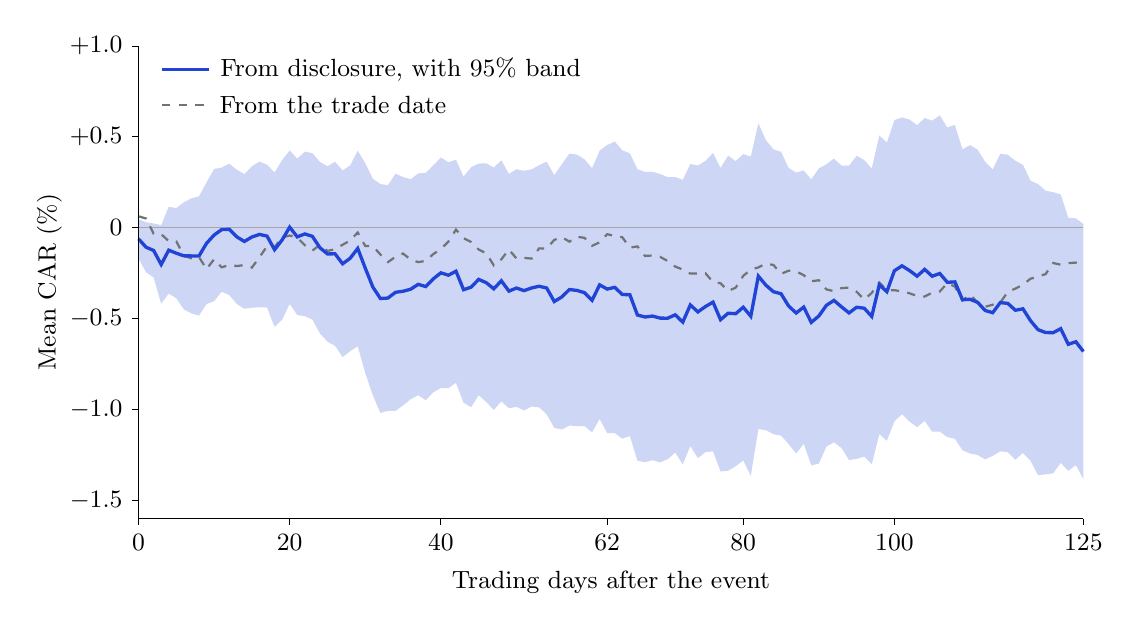
\begin{tikzpicture}[font=\small]
  \fill[accent!22] (0.000,3.802) -- (0.096,3.763) -- (0.192,3.747) -- (0.288,3.725) -- (0.384,3.959) -- (0.480,3.942) -- (0.576,4.016) -- (0.672,4.066) -- (0.768,4.092) -- (0.864,4.268) -- (0.960,4.439) -- (1.056,4.457) -- (1.152,4.507) -- (1.248,4.430) -- (1.344,4.374) -- (1.440,4.473) -- (1.536,4.533) -- (1.632,4.494) -- (1.728,4.394) -- (1.824,4.551) -- (1.920,4.675) -- (2.016,4.570) -- (2.112,4.659) -- (2.208,4.640) -- (2.304,4.528) -- (2.400,4.474) -- (2.496,4.531) -- (2.592,4.420) -- (2.688,4.484) -- (2.784,4.672) -- (2.880,4.513) -- (2.976,4.316) -- (3.072,4.247) -- (3.168,4.234) -- (3.264,4.379) -- (3.360,4.336) -- (3.456,4.308) -- (3.552,4.383) -- (3.648,4.389) -- (3.744,4.485) -- (3.840,4.585) -- (3.936,4.524) -- (4.032,4.557) -- (4.128,4.342) -- (4.224,4.461) -- (4.320,4.508) -- (4.416,4.510) -- (4.512,4.457) -- (4.608,4.549) -- (4.704,4.377) -- (4.800,4.436) -- (4.896,4.416) -- (4.992,4.434) -- (5.088,4.487) -- (5.184,4.532) -- (5.280,4.361) -- (5.376,4.499) -- (5.472,4.634) -- (5.568,4.622) -- (5.664,4.562) -- (5.760,4.449) -- (5.856,4.671) -- (5.952,4.743) -- (6.048,4.788) -- (6.144,4.676) -- (6.240,4.638) -- (6.336,4.437) -- (6.432,4.402) -- (6.528,4.402) -- (6.624,4.376) -- (6.720,4.336) -- (6.816,4.337) -- (6.912,4.301) -- (7.008,4.502) -- (7.104,4.483) -- (7.200,4.542) -- (7.296,4.643) -- (7.392,4.452) -- (7.488,4.609) -- (7.584,4.538) -- (7.680,4.628) -- (7.776,4.596) -- (7.872,5.020) -- (7.968,4.805) -- (8.064,4.689) -- (8.160,4.656) -- (8.256,4.453) -- (8.352,4.394) -- (8.448,4.421) -- (8.544,4.307) -- (8.640,4.446) -- (8.736,4.499) -- (8.832,4.571) -- (8.928,4.482) -- (9.024,4.481) -- (9.120,4.607) -- (9.216,4.554) -- (9.312,4.444) -- (9.408,4.865) -- (9.504,4.774) -- (9.600,5.060) -- (9.696,5.093) -- (9.792,5.067) -- (9.888,4.995) -- (9.984,5.087) -- (10.080,5.053) -- (10.176,5.120) -- (10.272,4.966) -- (10.368,4.999) -- (10.464,4.690) -- (10.560,4.742) -- (10.656,4.685) -- (10.752,4.532) -- (10.848,4.433) -- (10.944,4.632) -- (11.040,4.620) -- (11.136,4.543) -- (11.232,4.492) -- (11.328,4.292) -- (11.424,4.247) -- (11.520,4.163) -- (11.616,4.145) -- (11.712,4.115) -- (11.808,3.820) -- (11.904,3.812) -- (12.000,3.741) -- (12.000,0.501) -- (11.904,0.678) -- (11.808,0.606) -- (11.712,0.707) -- (11.616,0.574) -- (11.520,0.561) -- (11.424,0.550) -- (11.328,0.734) -- (11.232,0.833) -- (11.136,0.746) -- (11.040,0.844) -- (10.944,0.852) -- (10.848,0.796) -- (10.752,0.752) -- (10.656,0.807) -- (10.560,0.826) -- (10.464,0.867) -- (10.368,1.012) -- (10.272,1.034) -- (10.176,1.104) -- (10.080,1.102) -- (9.984,1.241) -- (9.888,1.161) -- (9.792,1.231) -- (9.696,1.325) -- (9.600,1.234) -- (9.504,0.988) -- (9.408,1.071) -- (9.312,0.689) -- (9.216,0.787) -- (9.120,0.758) -- (9.024,0.742) -- (8.928,0.895) -- (8.832,0.968) -- (8.736,0.914) -- (8.640,0.697) -- (8.544,0.674) -- (8.448,0.950) -- (8.352,0.826) -- (8.256,0.946) -- (8.160,1.053) -- (8.064,1.071) -- (7.968,1.122) -- (7.872,1.136) -- (7.776,0.542) -- (7.680,0.738) -- (7.584,0.664) -- (7.488,0.606) -- (7.392,0.598) -- (7.296,0.853) -- (7.200,0.843) -- (7.104,0.766) -- (7.008,0.921) -- (6.912,0.688) -- (6.816,0.837) -- (6.720,0.753) -- (6.624,0.713) -- (6.528,0.741) -- (6.432,0.715) -- (6.336,0.734) -- (6.240,1.047) -- (6.144,1.014) -- (6.048,1.085) -- (5.952,1.085) -- (5.856,1.264) -- (5.760,1.094) -- (5.664,1.174) -- (5.568,1.173) -- (5.472,1.181) -- (5.376,1.130) -- (5.280,1.152) -- (5.184,1.322) -- (5.088,1.412) -- (4.992,1.422) -- (4.896,1.373) -- (4.800,1.418) -- (4.704,1.399) -- (4.608,1.488) -- (4.512,1.378) -- (4.416,1.480) -- (4.320,1.565) -- (4.224,1.414) -- (4.128,1.470) -- (4.032,1.724) -- (3.936,1.655) -- (3.840,1.656) -- (3.744,1.603) -- (3.648,1.503) -- (3.552,1.566) -- (3.456,1.515) -- (3.360,1.437) -- (3.264,1.367) -- (3.168,1.367) -- (3.072,1.341) -- (2.976,1.564) -- (2.880,1.846) -- (2.784,2.187) -- (2.688,2.125) -- (2.592,2.050) -- (2.496,2.193) -- (2.400,2.245) -- (2.304,2.350) -- (2.208,2.527) -- (2.112,2.570) -- (2.016,2.584) -- (1.920,2.725) -- (1.824,2.525) -- (1.728,2.434) -- (1.632,2.679) -- (1.536,2.682) -- (1.440,2.677) -- (1.344,2.664) -- (1.248,2.724) -- (1.152,2.839) -- (1.056,2.880) -- (0.960,2.761) -- (0.864,2.723) -- (0.768,2.576) -- (0.672,2.605) -- (0.576,2.656) -- (0.480,2.796) -- (0.384,2.857) -- (0.288,2.727) -- (0.192,3.062) -- (0.096,3.127) -- (0.000,3.301) -- cycle;
  \draw[gray!70] (0,3.692) -- (12.0,3.692);
  \draw[black!55, dashed, line width=0.8pt] (0.000,3.838) -- (0.096,3.810) -- (0.192,3.619) -- (0.288,3.612) -- (0.384,3.523) -- (0.480,3.519) -- (0.576,3.340) -- (0.672,3.304) -- (0.768,3.321) -- (0.864,3.167) -- (0.960,3.293) -- (1.056,3.190) -- (1.152,3.220) -- (1.248,3.207) -- (1.344,3.218) -- (1.440,3.187) -- (1.536,3.318) -- (1.632,3.457) -- (1.728,3.447) -- (1.824,3.569) -- (1.920,3.594) -- (2.016,3.568) -- (2.112,3.471) -- (2.208,3.403) -- (2.304,3.475) -- (2.400,3.398) -- (2.496,3.420) -- (2.592,3.477) -- (2.688,3.530) -- (2.784,3.633) -- (2.880,3.461) -- (2.976,3.460) -- (3.072,3.353) -- (3.168,3.256) -- (3.264,3.324) -- (3.360,3.365) -- (3.456,3.288) -- (3.552,3.256) -- (3.648,3.272) -- (3.744,3.358) -- (3.840,3.423) -- (3.936,3.517) -- (4.032,3.669) -- (4.128,3.560) -- (4.224,3.512) -- (4.320,3.416) -- (4.416,3.369) -- (4.512,3.215) -- (4.608,3.292) -- (4.704,3.416) -- (4.800,3.303) -- (4.896,3.310) -- (4.992,3.301) -- (5.088,3.431) -- (5.184,3.429) -- (5.280,3.538) -- (5.376,3.574) -- (5.472,3.516) -- (5.568,3.578) -- (5.664,3.565) -- (5.760,3.463) -- (5.856,3.508) -- (5.952,3.611) -- (6.048,3.588) -- (6.144,3.572) -- (6.240,3.440) -- (6.336,3.456) -- (6.432,3.335) -- (6.528,3.340) -- (6.624,3.323) -- (6.720,3.270) -- (6.816,3.200) -- (6.912,3.161) -- (7.008,3.110) -- (7.104,3.113) -- (7.200,3.115) -- (7.296,3.003) -- (7.392,2.988) -- (7.488,2.890) -- (7.584,2.932) -- (7.680,3.082) -- (7.776,3.161) -- (7.872,3.189) -- (7.968,3.237) -- (8.064,3.220) -- (8.160,3.107) -- (8.256,3.147) -- (8.352,3.139) -- (8.448,3.090) -- (8.544,3.013) -- (8.640,3.026) -- (8.736,2.910) -- (8.832,2.887) -- (8.928,2.926) -- (9.024,2.933) -- (9.120,2.880) -- (9.216,2.780) -- (9.312,2.865) -- (9.408,2.998) -- (9.504,2.898) -- (9.600,2.899) -- (9.696,2.885) -- (9.792,2.860) -- (9.888,2.826) -- (9.984,2.820) -- (10.080,2.868) -- (10.176,2.883) -- (10.272,2.990) -- (10.368,2.946) -- (10.464,2.768) -- (10.560,2.845) -- (10.656,2.743) -- (10.752,2.689) -- (10.848,2.715) -- (10.944,2.742) -- (11.040,2.879) -- (11.136,2.920) -- (11.232,2.969) -- (11.328,3.045) -- (11.424,3.072) -- (11.520,3.104) -- (11.616,3.245) -- (11.712,3.223) -- (11.808,3.243) -- (11.904,3.250) -- (12.000,3.222);
  \draw[accent, line width=1.2pt] (0.000,3.552) -- (0.096,3.445) -- (0.192,3.404) -- (0.288,3.226) -- (0.384,3.408) -- (0.480,3.369) -- (0.576,3.336) -- (0.672,3.335) -- (0.768,3.334) -- (0.864,3.495) -- (0.960,3.600) -- (1.056,3.669) -- (1.152,3.673) -- (1.248,3.577) -- (1.344,3.519) -- (1.440,3.575) -- (1.536,3.608) -- (1.632,3.587) -- (1.728,3.414) -- (1.824,3.538) -- (1.920,3.700) -- (2.016,3.577) -- (2.112,3.614) -- (2.208,3.584) -- (2.304,3.439) -- (2.400,3.360) -- (2.496,3.362) -- (2.592,3.235) -- (2.688,3.305) -- (2.784,3.430) -- (2.880,3.179) -- (2.976,2.940) -- (3.072,2.794) -- (3.168,2.800) -- (3.264,2.873) -- (3.360,2.886) -- (3.456,2.912) -- (3.552,2.974) -- (3.648,2.946) -- (3.744,3.044) -- (3.840,3.120) -- (3.936,3.090) -- (4.032,3.141) -- (4.128,2.906) -- (4.224,2.938) -- (4.320,3.037) -- (4.416,2.995) -- (4.512,2.917) -- (4.608,3.019) -- (4.704,2.888) -- (4.800,2.927) -- (4.896,2.894) -- (4.992,2.928) -- (5.088,2.950) -- (5.184,2.927) -- (5.280,2.756) -- (5.376,2.814) -- (5.472,2.908) -- (5.568,2.897) -- (5.664,2.868) -- (5.760,2.771) -- (5.856,2.967) -- (5.952,2.914) -- (6.048,2.936) -- (6.144,2.845) -- (6.240,2.842) -- (6.336,2.585) -- (6.432,2.559) -- (6.528,2.571) -- (6.624,2.545) -- (6.720,2.544) -- (6.816,2.587) -- (6.912,2.494) -- (7.008,2.712) -- (7.104,2.624) -- (7.200,2.692) -- (7.296,2.748) -- (7.392,2.525) -- (7.488,2.607) -- (7.584,2.601) -- (7.680,2.683) -- (7.776,2.569) -- (7.872,3.078) -- (7.968,2.963) -- (8.064,2.880) -- (8.160,2.855) -- (8.256,2.699) -- (8.352,2.610) -- (8.448,2.685) -- (8.544,2.491) -- (8.640,2.572) -- (8.736,2.707) -- (8.832,2.770) -- (8.928,2.688) -- (9.024,2.611) -- (9.120,2.683) -- (9.216,2.671) -- (9.312,2.566) -- (9.408,2.968) -- (9.504,2.881) -- (9.600,3.147) -- (9.696,3.209) -- (9.792,3.149) -- (9.888,3.078) -- (9.984,3.164) -- (10.080,3.077) -- (10.176,3.112) -- (10.272,3.000) -- (10.368,3.005) -- (10.464,2.779) -- (10.560,2.784) -- (10.656,2.746) -- (10.752,2.642) -- (10.848,2.614) -- (10.944,2.742) -- (11.040,2.732) -- (11.136,2.645) -- (11.232,2.663) -- (11.328,2.513) -- (11.424,2.398) -- (11.520,2.362) -- (11.616,2.360) -- (11.712,2.411) -- (11.808,2.213) -- (11.904,2.245) -- (12.000,2.121);
  \draw (0,0) -- (12.0,0);
  \draw (0,0) -- (0,6.0);
  \draw (0.000,0) -- (0.000,-0.08) node[below] {0};
  \draw (1.920,0) -- (1.920,-0.08) node[below] {20};
  \draw (3.840,0) -- (3.840,-0.08) node[below] {40};
  \draw (5.952,0) -- (5.952,-0.08) node[below] {62};
  \draw (7.680,0) -- (7.680,-0.08) node[below] {80};
  \draw (9.600,0) -- (9.600,-0.08) node[below] {100};
  \draw (12.000,0) -- (12.000,-0.08) node[below] {125};
  \draw (0,0.231) -- (-0.08,0.231) node[left] {$-1.5$};
  \draw (0,1.385) -- (-0.08,1.385) node[left] {$-1.0$};
  \draw (0,2.538) -- (-0.08,2.538) node[left] {$-0.5$};
  \draw (0,3.692) -- (-0.08,3.692) node[left] {0};
  \draw (0,4.846) -- (-0.08,4.846) node[left] {$+0.5$};
  \draw (0,6.000) -- (-0.08,6.000) node[left] {$+1.0$};
  \node[below] at (6.0,-0.55) {Trading days after the event};
  \node[rotate=90, above] at (-0.85,3.0) {Mean CAR (\%)};
  \draw[accent, line width=1.2pt] (0.3,5.70) -- (0.9,5.70) node[right, black] {From disclosure, with 95\% band};
  \draw[black!55, dashed, line width=0.8pt] (0.3,5.25) -- (0.9,5.25) node[right, black] {From the trade date};
\end{tikzpicture}

\caption{Mean cumulative four-factor abnormal return over days $[0, d]$ for each trading day $d$ after the event. The solid line and band use the disclosure date as day 0; the dashed line uses the transaction date. The band is a pointwise 95\% interval and covers zero on every day. Each day's mean uses the events observed through that day, so the sample shrinks as events reach the end of the data (3,869 disclosure-date events on day 0, 3,139 on day 125).}\label{fig:car}
\end{figure}

\subsection{Robustness}

None of the plan's alternative samples or weighting schemes produces a statistically significant alpha (Table~\ref{tab:robust}). Dropping trades made in 2020 (\m3.60\%, $t = \m1.49$), dropping the five most active members (\m3.07\%, $t = \m1.12$) and keeping only members' own trades (\m5.00\%, $t = \m1.51$) all move the estimate down. Weighting each stock by the disclosed amounts of its active purchases moves it up, to 7.19\% a year ($t = 1.45$). Tested directly, the difference between the amount-weighted and the equal-weighted portfolio has an alpha of 8.83\% a year ($t = 1.65$, $p = 0.099$; Table~\ref{tab:extra}). That is the one hint in the data that larger purchases do better, and it is not significant at the 5\% level. Senate purchases, measured from the trade date, give \m0.95\% ($t = \m0.10$) on only 288 portfolio days. Stocks that members sold, held long from the disclosure of the sale, earn +0.95\% ($t = 0.34$), so sold stocks do not underperform either. This is not the return to imitating the sale, which would mean shorting the stock.

\begin{table}[t]
\centering
\caption{Robustness of the primary test ($H = 62$, four-factor alpha)}\label{tab:robust}
\begin{tabular}{lrrrrr}
\toprule
Sample or weighting & Events & Alpha (annual) & $t$ & $p$ & Days \\
\midrule
Primary: House purchases from disclosure & 3,942 & \m1.63\% & \m0.66 & 0.509 & 1,505 \\
Leave out trades made in 2020 & 3,234 & \m3.60\% & \m1.49 & 0.137 & 1,252 \\
Drop the five most active members & 2,622 & \m3.07\% & \m1.12 & 0.261 & 1,505 \\
Weight by disclosed amount & 3,942 & 7.19\% & 1.45 & 0.148 & 1,505 \\
Members' own trades only & 1,861 & \m5.00\% & \m1.51 & 0.131 & 1,496 \\
House purchases from the trade date & 3,996 & \m1.38\% & \m0.59 & 0.557 & 1,507 \\
Senate purchases from the trade date & 460 & \m0.95\% & \m0.10 & 0.920 & 288 \\
Stocks sold, held long from disclosure & 4,284 & 0.95\% & 0.34 & 0.736 & 1,502 \\
\bottomrule
\end{tabular}

\smallskip
\parbox{0.9\linewidth}{\footnotesize Each row reruns the calendar-time regression of Table~\ref{tab:calendar}. Under amount weighting, a stock's weight on a day is the sum, over its active purchases, of the midpoint of each disclosed band (or its floor when the band is open-ended); otherwise weights are equal by stock. Trade-date rows enter on the first trading day after the trade. ``Own trades'' excludes trades owned by a spouse, a dependent child, or jointly.}
\end{table}

\begin{table}[t]
\centering
\caption{Further checks: the planned five-factor model and analyses added after review}\label{tab:extra}
\begin{tabular}{lrrrrr}
\toprule
\multicolumn{6}{l}{\textit{Copy portfolio alpha (annual), 1,505 portfolio days}} \\
Check & $H$ & Alpha & $t$ & $p$ & \\
\midrule
Five-factor model & 20 & 2.37\% & 0.75 & 0.456 & \\
Five-factor model & 62 & \m1.25\% & \m0.53 & 0.597 & \\
Five-factor model & 125 & \m1.33\% & \m0.62 & 0.536 & \\
Newey--West, 21 lags & 62 & \m1.63\% & \m0.71 & 0.479 & \\
Newey--West, 62 lags & 62 & \m1.63\% & \m0.75 & 0.454 & \\
Amount-weighted minus equal-weighted & 62 & 8.83\% & 1.65 & 0.099 & \\
\midrule
\multicolumn{6}{l}{\textit{Event-level four-factor abnormal returns, House purchases}} \\
Window & Events & Mean & s.e. & $t$ & $p$ \\
\midrule
Holding window, days 1--20 & 3,795 & 0.05\% & 0.22\% & 0.25 & 0.802 \\
Holding window, days 1--62 & 3,630 & \m0.27\% & 0.42\% & \m0.64 & 0.521 \\
Holding window, days 1--125 & 3,141 & \m0.62\% & 0.38\% & \m1.64 & 0.101 \\
Trade to the copier's entry & 3,863 & \m0.24\% & 0.12\% & \m1.99 & 0.046 \\
\bottomrule
\end{tabular}

\smallskip
\parbox{0.9\linewidth}{\footnotesize The five-factor model is \citet{fama2015five}, without momentum. ``Amount-weighted minus equal-weighted'' regresses the daily difference between the two 62-day portfolios on the four factors. Holding-window CARs start on the first trading day after the disclosure date; their Holm-adjusted p-values across the three horizons are 1.000, 1.000 and 0.302. The trade-to-entry window runs from the trade's day 0 to the last trading day before entry (median 11 trading days), with loadings estimated before the trade. Only the five-factor model was in the plan; the rest were added after an outside review and are exploratory.}
\end{table}

\subsection{Members buy stocks that had been beating the model}\label{sec:runup}

The first run's significantly negative CARs (Appendix Table~\ref{tab:firstrun}) come from one term. That run subtracted each stock's estimated pre-event intercept, its average four-factor abnormal return over days $-250$ to $-30$, on every day of the event window. For the disclosure-date events that intercept, scaled to 63 trading days, has a mean of +1.67\% and a median of +0.79\%, and it is positive for 55\% of events. Subtracting it assumes the stock will keep beating the model at its past rate; when the stock instead earns its factor-predicted return, the CAR comes out negative. With betas only, the CARs agree with the calendar-time test, which has no pre-event intercept at all. The event-level results are therefore sensitive to how abnormal returns are specified, while the calendar-time test, which needs no pre-event estimate, is not; that is one reason it is the primary test.

This pattern is exploratory, and it is the opposite of \citet{belmont2020relief}, who report that stocks senators bought had underperformed in the 100 days before purchase. It suggests that House members in this period tended to buy stocks after a stretch of factor-adjusted gains, and that those stocks did not continue to outperform.

\section{How long members take to disclose}\label{sec:lag}

Table~\ref{tab:lag} and Figure~\ref{fig:lag} describe disclosure delays for House trades of every transaction type in the snapshot from 2020 to 2025. Of the snapshot's 16,202 rows, 15,193 remain after duplicates are removed and 14,109 have a transaction date in that period; setting aside the rows listed under the table leaves 12,650 trades, all from the House. The legal deadline is the earlier of 30 days after the filer learns of a transaction and 45 days after it. The snapshot has no notification dates, so only the 45-day outer limit can be checked: a trade counts as past the limit when it was disclosed more than 45 days after the transaction date, and a filing counts when it lists at least one such trade. Some trades disclosed within 45 days may still have missed the 30-day rule, so these counts are a lower bound on late reporting. Most trades are disclosed well within the outer limit: the median delay is 13 days overall and between 8 and 22 days in every year. Across the six years, 833 of 12,650 trades (6.6\%) were disclosed more than 45 days after the trade, in 69 of 1,965 filings, by 48 of 210 members.

These trades cluster in a few filings. In 2024, 217 of them come from 14 filings, one of which lists 68; in 2025 a single filing lists 234. Trade counts therefore overstate how often members file past the limit, and the filing counts are the better measure. Two caveats apply. The snapshot does not mark amendments, so some of these trades may have been reported on time and re-listed in an amended filing. And filings for late-2025 trades made after the snapshot was taken in April 2026 are missing, so the 2025 share over 45 days is a lower bound.

\begin{table}[t]
\centering
\caption{Disclosure delay of House trades, by transaction year}\label{tab:lag}
\begin{tabular}{lrrrrrrr}
\toprule
Year & Trades & Median days & 90th pct. & Over 45 days & Share & Filings & Filings over 45 \\
\midrule
2020 & 2,678 & 9 & 31 & 73 & 2.7\% & 488 & 24 \\
2021 & 2,047 & 8 & 32 & 59 & 2.9\% & 398 & 17 \\
2022 & 1,405 & 8 & 32 & 6 & 0.4\% & 308 & 4 \\
2023 & 1,816 & 22 & 31 & 95 & 5.2\% & 255 & 11 \\
2024 & 1,203 & 17 & 292 & 217 & 18.0\% & 238 & 14 \\
2025 & 3,501 & 14 & 50 & 383 & 10.9\% & 318 & 9 \\
All & 12,650 & 13 & 34 & 833 & 6.6\% & 1,965 & 69 \\
\bottomrule
\end{tabular}

\smallskip
\parbox{0.92\linewidth}{\footnotesize All House transaction types, duplicates removed. ``Over 45 days'' counts trades disclosed more than 45 days after the trade, the statute's outer limit; the 30-day rule from notification cannot be checked. Yearly filing counts, and yearly counts of filings over 45 days, add to more than the totals (1,965 and 69) because a filing can list trades from two years. Excluded before tabulating: 1,325 trades with no disclosure date (mostly Senate rows), 34 dated before the trade and 100 dated more than 365 days after it.}
\end{table}

\begin{figure}[t]
\centering
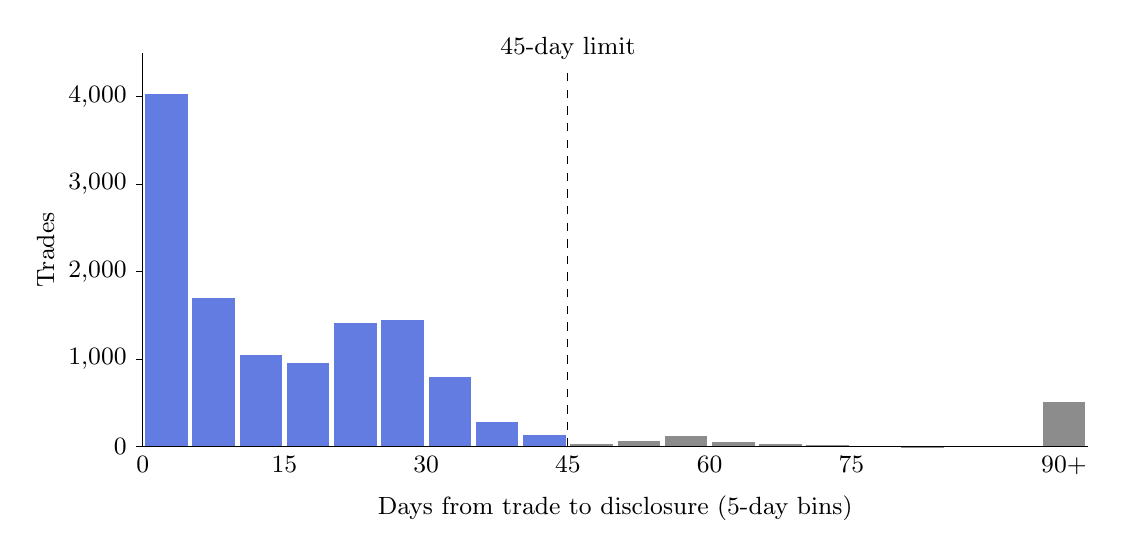
\begin{tikzpicture}[font=\small]
  \fill[accent!70] (0.030,0) rectangle (0.570,4.484);
  \fill[accent!70] (0.630,0) rectangle (1.170,1.893);
  \fill[accent!70] (1.230,0) rectangle (1.770,1.163);
  \fill[accent!70] (1.830,0) rectangle (2.370,1.062);
  \fill[accent!70] (2.430,0) rectangle (2.970,1.566);
  \fill[accent!70] (3.030,0) rectangle (3.570,1.612);
  \fill[accent!70] (3.630,0) rectangle (4.170,0.881);
  \fill[accent!70] (4.230,0) rectangle (4.770,0.312);
  \fill[accent!70] (4.830,0) rectangle (5.370,0.144);
  \fill[black!45] (5.430,0) rectangle (5.970,0.032);
  \fill[black!45] (6.030,0) rectangle (6.570,0.071);
  \fill[black!45] (6.630,0) rectangle (7.170,0.132);
  \fill[black!45] (7.230,0) rectangle (7.770,0.056);
  \fill[black!45] (7.830,0) rectangle (8.370,0.040);
  \fill[black!45] (8.430,0) rectangle (8.970,0.019);
  \fill[black!45] (9.030,0) rectangle (9.570,0.008);
  \fill[black!45] (9.630,0) rectangle (10.170,0.003);
  \fill[black!45] (10.230,0) rectangle (10.770,0.009);
  \fill[black!45] (11.430,0) rectangle (11.970,0.567);
  \node[below] at (11.700,0) {90+};
  \draw (0,0) -- (12.0,0);
  \draw (0,0) -- (0,5.0);
  \draw[dashed] (5.400,0) -- (5.400,4.80) node[above] {45-day limit};
  \node[below] at (0.000,0) {0};
  \node[below] at (1.800,0) {15};
  \node[below] at (3.600,0) {30};
  \node[below] at (5.400,0) {45};
  \node[below] at (7.200,0) {60};
  \node[below] at (9.000,0) {75};
  \draw (0,0.000) -- (-0.08,0.000) node[left] {0};
  \draw (0,1.111) -- (-0.08,1.111) node[left] {1,000};
  \draw (0,2.222) -- (-0.08,2.222) node[left] {2,000};
  \draw (0,3.333) -- (-0.08,3.333) node[left] {3,000};
  \draw (0,4.444) -- (-0.08,4.444) node[left] {4,000};
  \node[below] at (6.0,-0.5) {Days from trade to disclosure (5-day bins)};
  \node[rotate=90, above] at (-1.0,2.5) {Trades};
\end{tikzpicture}

\caption{Days from trade to disclosure for 12,650 House trades, 2020--2025. Blue bars are within the 45-day outer limit. The last bar collects delays of 90 days or more.}\label{fig:lag}
\end{figure}

\section{Discussion and limitations}\label{sec:discussion}

The primary estimate is negative but imprecise. Its 95\% confidence interval runs from \m6.48\% to +3.22\% a year, so the data are inconsistent with copying disclosed House purchases from 2020 to 2025 having earned more than about 3.2\% a year above its factor exposures, and the strategy may have earned less than the factors predict. The result is consistent with \citet{eggers2013capitol}, \citet{belmont2020relief} and \citet{fischer2025democracy}, who find no significant outperformance from the trade date, and extends that finding to the returns an outside investor could act on.

A null result for copying does not establish that no member trades on private information. Individual trades, members or committees could earn abnormal returns that an average over 3,942 purchases hides, and the amount-weighted estimate leaves room for larger trades to do somewhat better. The data cannot separate information from luck or from ordinary portfolio choices, and this paper makes no claim about insider trading.

Several limitations affect the interpretation of these results:
\begin{itemize}
\item \textbf{House only.} The primary test excludes the Senate because the snapshot has no Senate disclosure dates. The Senate's trade-date estimate rests on 460 purchases.
\item \textbf{One snapshot.} The trades come from a third-party transcription, not a fresh collection from the official filings, and cannot be re-downloaded from the same source. A replication against the official records would test its accuracy.
\item \textbf{Disclosure date as recorded.} The disclosure date is the date in the snapshot. If a filing became publicly visible later than that date, the true copy strategy would enter later.
\item \textbf{Common stock only.} Exchange-traded funds, ADRs, foreign over-the-counter shares and options are excluded, and they are a meaningful share of members' trading.
\item \textbf{No costs.} Returns ignore trading costs, which would lower the copy strategy's return further.
\item \textbf{Censoring.} CRSP data end on 31 December 2025. Long-horizon CARs omit purchases from about mid-2025; in the 62-day portfolio, 39 purchases never enter and 237 are held for fewer than 62 days.
\end{itemize}

\section{Conclusion}

From 2020 to 2025, an investor who bought what House members bought, on the day after each purchase was disclosed, would have earned roughly the return that the stocks' exposure to the market, size, value and momentum factors predicts. The primary four-factor alpha is \m1.63\% a year and insignificant, the event-level abnormal returns are insignificant from both the trade and the disclosure date, and the robustness checks agree. Members mostly disclose within the 45-day outer limit, and disclosures past it are concentrated in a few filings.

\section*{Data and code availability}

Code, the trade snapshot, the sample-flow output and the aggregate figures are in the project repository at \url{https://github.com/Builder106/capitol-alpha} under the MIT license. The plan is \texttt{docs/specs/event-study.md}, and its commit history shows when each part was fixed. CRSP data are licensed through Wharton Research Data Services and are not redistributed; a reader with CRSP access can rebuild every table with \texttt{pipeline.crsp} and \texttt{pipeline.run\_event\_study}, which stops at the 31 December 2025 cutoff. The Zenodo record links the exact commit of the code that produced these tables. The factors are public \citep{french2026data}.

\section*{Declarations}

\noindent\textbf{Funding.} This research received no specific grant from any funding agency in the public, commercial or not-for-profit sectors. CRSP data were accessed through Wesleyan University's subscription to Wharton Research Data Services.

\medskip
\noindent\textbf{Competing interests.} I declare no competing interests.

\medskip
\noindent\textbf{Use of AI tools.} I used Claude (Anthropic) to assist with writing the manuscript and the analysis code. I reviewed all text, code and results and take full responsibility for the content of this paper.

\bibliographystyle{plainnat}
\bibliography{references}

\appendix
\section{The first run, with the pre-event intercept}

\begin{table}[H]
\centering
\caption{First run: CARs that also subtract the pre-event intercept}\label{tab:firstrun}
\begin{tabular}{lrrrrrrr}
\toprule
Event date & Days & Events & Mean CAR & s.e. & $t$ & $p$ & Holm $p$ \\
\midrule
Disclosure & 20 & 3,795 & \m0.56\% & 0.22\% & \m2.59 & 0.010 & 0.011 \\
Disclosure & 62 & 3,630 & \m1.98\% & 0.51\% & \m3.87 & $<$0.001 & $<$0.001 \\
Disclosure & 125 & 3,139 & \m4.43\% & 0.96\% & \m4.61 & $<$0.001 & $<$0.001 \\
Transaction & 20 & 4,372 & \m0.63\% & 0.23\% & \m2.78 & 0.005 & 0.011 \\
Transaction & 62 & 4,161 & \m1.76\% & 0.45\% & \m3.88 & $<$0.001 & $<$0.001 \\
Transaction & 125 & 3,931 & \m3.80\% & 0.74\% & \m5.13 & $<$0.001 & $<$0.001 \\
\bottomrule
\end{tabular}

\smallskip
\parbox{0.9\linewidth}{\footnotesize Same as Table~\ref{tab:cars}, except that the expected return also includes the stock's intercept from days $-250$ to $-30$. This was the first run; the plan specifies betas only. See Section~\ref{sec:runup}.}
\end{table}

\section{Relation to an earlier version of this project}\label{app:earlier}

An earlier version of this project, presented on its website and in the author's materials, reported that copying Senate purchases earned 2.58\% more than the SPY index fund over 90 days ($p = 0.013$, $n = 220$). An audit found that the estimate dropped every House purchase through a coding error, priced only the 50 most-traded tickers, measured returns from the transaction date, adjusted for risk by subtracting the index return, and treated overlapping trades as independent. That estimate is withdrawn. This paper replaces it, and the plan described in Section~\ref{sec:plan} was written to prevent the same problems.

\end{document}
